\section{Conception}

\subsection{Délimitation fonctionnelle}

La section suivante est un rappel de la délimitation du circuit à concevoir. Celle-ci présente le contrôleur d'interruptions d'un point de vue extérieur avec les 6 relations définies précédemment.

\begin{figure}[H]
	\centering
	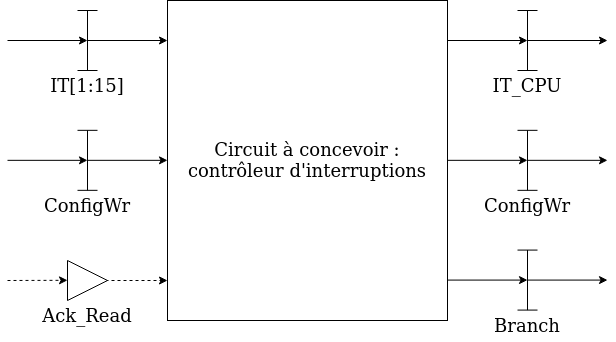
\includegraphics[width=0.6\linewidth]{figure/delimitation_fonctionnelle.png}
	\caption{Délimitation fonctionnelle du contrôleur d'interruptions}
	\label{fig:delimitation_fonctionnelle}
\end{figure}

Il s'agira par la suite de se placer dans un point de vue interne afin de présenter les différents blocs composant le contrôleur d'interruptions avec ses relations internes.
L'évènement \texttt{Ack\_Read} permet d'acquitter la lecture de l'adresse de branchement par le processeur. Cette relation peut être déduite selon le contenu du bus d'adresse (si la lecture est faite dans le registre \texttt{blx} alors il y a acquittement).  

\subsection{Décomposition fonctionnelle et introduction des interfaces}

La figure ci-dessous présente le circuit interne observé de l'intérieur avec l'introduction des signaux physiques du circuit. Il existe deux blocs nommés \texttt{Interface} et \texttt{Traitement}. 

\begin{figure}[H]
	\centering
	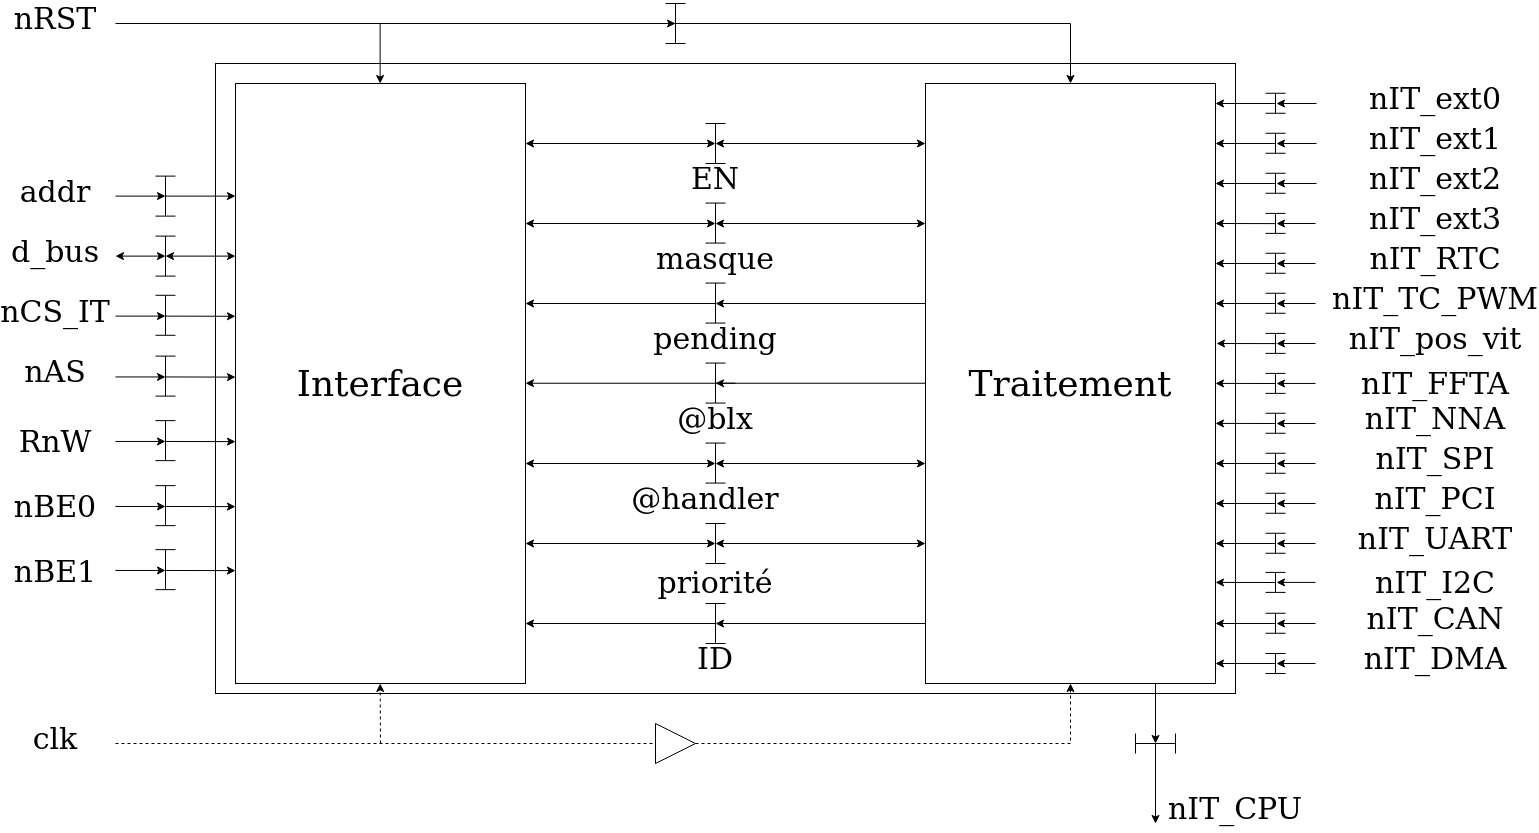
\includegraphics[width=1\linewidth]{figure/decomposition_fonctionnelle.png}
	\caption{Décomposition fonctionnelle et introduction des interfaces}
	\label{fig:decomposition_fonctionnelle}
\end{figure}

Le bloc \texttt{Traitement} est chargé de signaler le CPU d'une interruption à traiter à la suite de multiples opérations (traitement des priorités, opération de masquage, mise en suspens).
Le bloc \texttt{Interface} permet de faire la jonction entre les signaux de contrôle et bus du système à microprocesseur et l'IP à concevoir.
\texttt{Ack\_Read} est en sortie du bloc \texttt{Interface} et avertit le bloc \texttt{Traitement} de la lecture de l'adresse de branchement.
Il ne s'agit plus d'un événement mais d'une relation.
C'est une variable partagée qui engendrera une action sur niveau et non sur front.

\subsection{Raffinage du bloc \texttt{Interface}}

La section suivante présente un raffinage, c'est-à-dire de réaliser une seconde décomposition en se plaçant à l'intérieur du bloc \texttt{Interface}.
Ce bloc est composé de \texttt{Interface\_Write} et \texttt{Interface\_Read}. 

\begin{figure}[H]
	\centering
	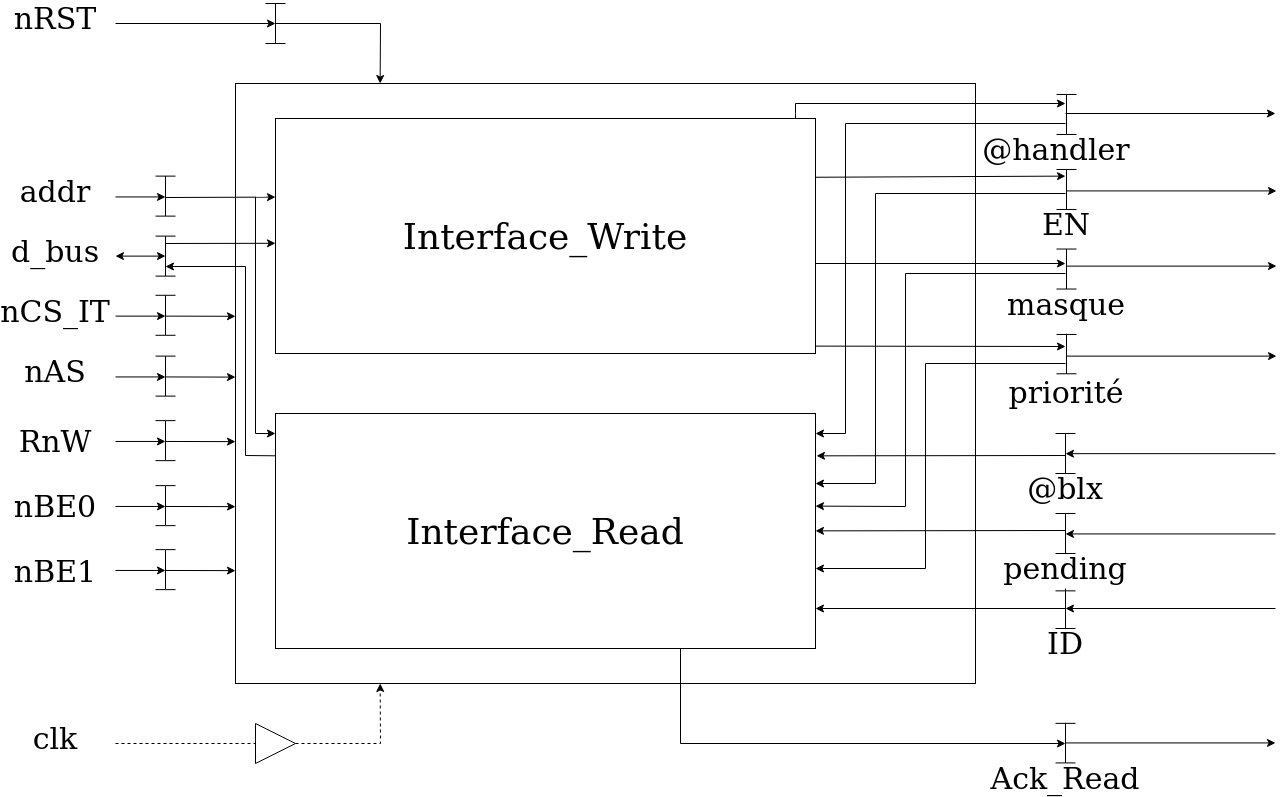
\includegraphics[width=1\linewidth]{figure/raffinage_interface.png}
	\caption{Raffinage et décomposition du bloc \texttt{Interface}}
	\label{fig:raffinage_interface}
\end{figure}

Cette décomposition en bloc hiérarchique permet de mettre en lumière deux fonctions du bloc \texttt{Interface}.
Celui-ci peut écrire dans les registres du contrôleur d'interruptions par le biais du bloc \texttt{Interface\_Write} et les lire avec \texttt{Interface\_Read}.

\subsection{Raffinage du bloc \texttt{Traitement}}

\begin{figure}[H]
	\centering
	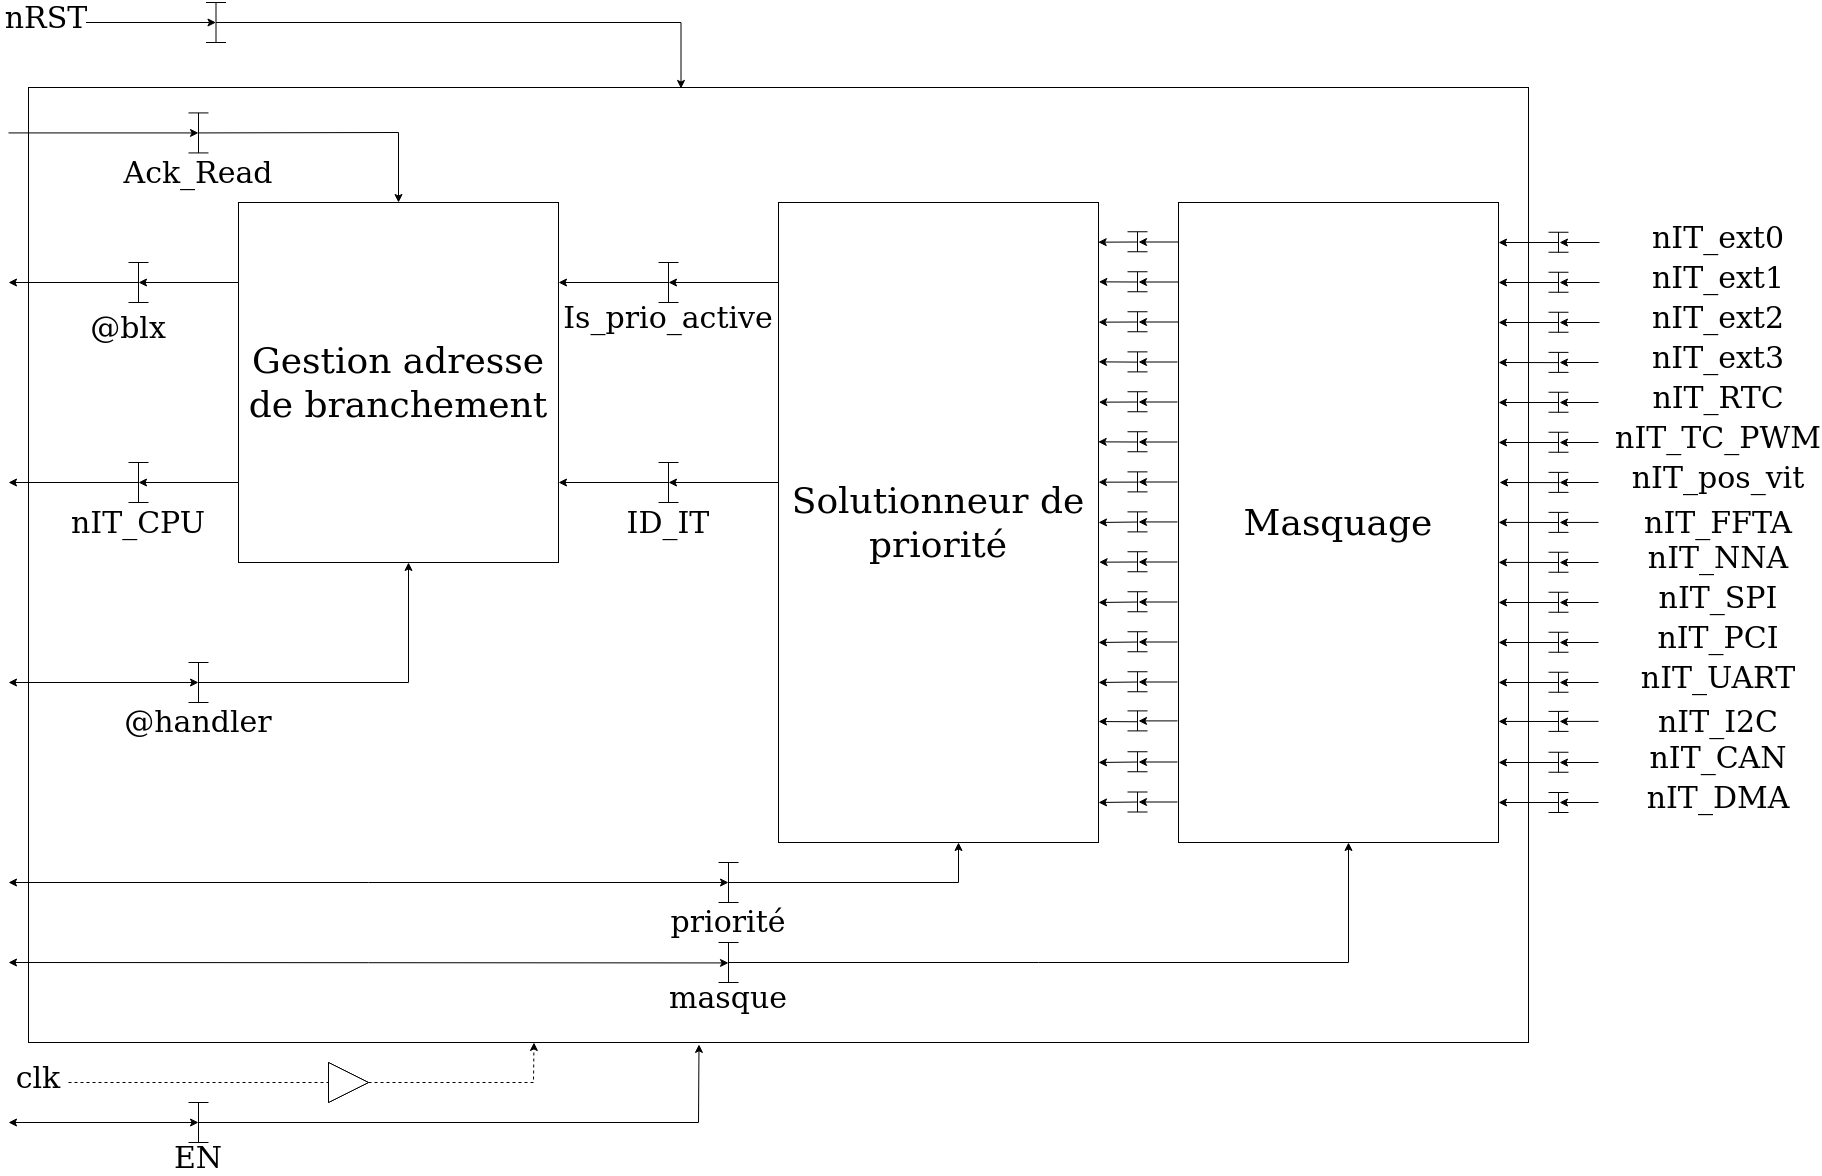
\includegraphics[width=1\linewidth]{figure/raffinage_traitement.png}
	\caption{Raffinage et décomposition du bloc \texttt{Traitement}}
	\label{fig:raffinage_traitement}
\end{figure}

\newpage

\subsection{Écriture des algorithmes}

\subsubsection{Algorithme \texttt{Interface\_Write}}

\begin{lstlisting}[style=pascalstyle]
action Interface_Write sur clk avec
(
entree var d_bus 			: Def_data;
entree var addr 			: Def_addr;
entree var nRST 			: Def_Bit
entree var nCS_IT 			: Def_Bit;
entree var nAS 				: Def_Bit;
entree var RnW 				: Def_Bit;
sortie var EN 				: Def_Bit;
sortie var vect_priorite 	: Def_vect_priorite;
sortie var vect_handler 	: Def_vect_handler;
sortie var masque 			: Def_masque
);

const addr_EN 				: Def_addr = 0x000000;
const addr_masque 			: Def_addr = 0x000002;
const addr_vect_handler 	: Def_addr = 0x00000A;
const addr_vect_priorite 	: Def_addr = 0x000044;

begin

cycle:
begin
	cycle H:
	begin
	if (nRST=0) then
		EN := 0;
		priorite := 0;
		vect_handler := 0;
		masque := 0;
	end if;
	if (nCS_IT=0) et (RnW=0) et (nAS=0) then
	case addr of
	addr_EN:
		EN := d_bus;
	addr_masque:
		masque := d_bus;
	addr_vect_handler:
		vect_handler := d_bus;
	addr_vect_priorite:
		vect_priorite := d_bus;
	end if;
	end cycle H;
end cycle;
end Interface_Write;
\end{lstlisting}

\newpage
\subsubsection{Algorithme \texttt{Interface\_Read}}

\begin{lstlisting}[style=pascalstyle]
action Interface_Read sur clk avec
(
entree var addr 			: Def_addr;
entree var nCS_IT 			: Def_Bit;
entree var nAS 				: Def_Bit;
entree var RnW 				: Def_Bit;
entree var nRST 			: Def_Bit;
entree var EN 				: Def_Bit;
entree var vect_priorite 	: Def_vect_priorite;
entree var vect_handler 	: Def_vect_handler;
entree var masque 			: Def_masque;
entree var pending 			: Def_pending
entree var blx 				: Def_blx;
sortie var d_bus 			: Def_data
);

var TriState 				: HauteImpedance;
const addr_EN	     		: Def_addr = 0x000000;
const addr_masque   		: Def_addr = 0x000002;
const addr_pending 			: Def_addr = 0x000004;
const addr_blx 				: Def_addr = 0x000006;
const addr_vect_handler 	: Def_addr = 0x00000A;
const addr_vect_priorite 	: Def_addr = 0x000044;

begin

cycle:
begin
	cycle H:
	begin
	if (nRST=0) then
		//ne rien faire
	end if;
	d_bus := TriState;
	if (nCS_IT=0) et (RnW=1) et (nAS=0) then
		case addr of
		addr_EN:
			d_bus := EN;
		addr_masque:
			d_bus := masque;
		addr_vect_handler:
			d_bus := vect_handler;
		addr_vect_priorite:
			d_bus := vect_priorite;
		addr_pending:
			d_bus := pending;
		addr_blx:
			d_bus := blx;
	end if;
	end cycle H;
end cycle;
end Interface_Read;
\end{lstlisting}